\chapter{L'énergie cinétique et la sécurité routière}\label{ch:g9:kinetic-energy-safety}

Depuis les jouets à remontoir de ton enfance, l'\omterm{def:g5:everyday-energy:energy}{énergie} était une
histoire de réservoirs et de formes --- vivante, utile, et sans
chiffres. L'attente s'achève. L'\omterm{def:g5:everyday-energy:energy}{énergie} du mouvement reçoit sa
formule, l'\omterm{def:g5:everyday-energy:energy}{énergie} reçoit son \omterm{def:g6:measurement-in-science:measuring}{unité}, et l'arithmétique se trouve
gouverner une affaire de vie ou de mort~: pourquoi une voiture à
\omterm{def:g7:motion-average-speed:formula}{vitesse} double est quatre fois plus difficile à arrêter, et ce qu'une
seule seconde d'inattention coûte en \omterm{def:g2:measuring-length:units}{mètres}.

\section{L'énergie du mouvement}

\begin{definition}[Le joule]\label{def:g9:kinetic-energy-safety:joule}
L'\omterm{def:g5:everyday-energy:energy}{énergie} --- sous toutes ses formes --- se mesure en
\emph{joules}\index{joule} (\unit{J}), en l'honneur de
l'expérimentateur qui prouva que la \omterm{def:g5:heat-and-insulation:heat}{chaleur} elle-même est une forme
d'\omterm{def:g5:everyday-energy:energy}{énergie}. Repères~: soulever ce livre du sol à l'étagère dépense
quelques joules~; un cœur qui bat, environ un joule par battement~;
une tablette de chocolat garde en réserve un million de joules
d'\omterm{def:g5:everyday-energy:energy}{énergie} alimentaire.
\end{definition}

\begin{proposition}[Énergie cinétique]\label{prop:g9:kinetic-energy-safety:formula}
Un corps de \omterm{def:g3:measuring-mass:mass}{masse} $m$ (en \unit{kg}) qui se déplace à la \omterm{def:g7:motion-average-speed:formula}{vitesse} $v$
(en \unit{m/s}) porte, du seul fait de son mouvement,
l'\emph{énergie cinétique}\index{énergie cinétique}
\[
E_k = \frac{1}{2} \times m \times v^2 ,
\]
en \omterm{def:g9:kinetic-energy-safety:joule}{joules}. Deux réglages, deux puissances inégales~: doubler la \omterm{def:g3:measuring-mass:mass}{masse}
double $E_k$ --- mais doubler la \emph{\omterm{def:g7:motion-average-speed:formula}{vitesse}} la
\emph{quadruple}, car la \omterm{def:g7:motion-average-speed:formula}{vitesse} entre au carré. La \omterm{def:g7:motion-average-speed:formula}{vitesse} est le
réglage dangereux.
\end{proposition}

\begin{example}[Premiers calculs]\label{ex:g9:kinetic-energy-safety:first}
Un ballon de football de \qty{0.45}{kg} à \qty{20}{m/s}~:
$E_k = 0.5 \times 0.45 \times 20^2 = \qty{90}{J}$. Un sprinteur de
\qty{60}{kg} à \qty{10}{m/s}~:
$0.5 \times 60 \times 100 = \qty{3000}{J}$. Une voiture de
\qty{1000}{kg} à \qty{50}{km/h} --- convertir d'abord~:
$50 \div 3.6 \approx \qty{13.9}{m/s}$ ---
$E_k = 0.5 \times 1000 \times 13.9^2 \approx \qty{9.7e4}{J}$~: près
de cent mille \omterm{def:g9:kinetic-energy-safety:joule}{joules}. La même voiture à \qty{100}{km/h}~: quatre fois
plus --- \qty{3.9e5}{J}. L'avertissement de la formule, en nombres.
\end{example}

\begin{omfigure}
\begin{tikzpicture}
\begin{axis}[omaxis, width=10.2cm, height=6.0cm,
    xlabel={vitesse $v$ (\unit{km/h})},
    ylabel={$E_k$ (\unit{kJ})},
    xtick={0,30,50,70,90,110,130}, ytick={0,100,200,300,400,500},
    ymin=0, ymax=560, xmin=0, xmax=140, samples=100]
  \addplot[very thick, omThm, domain=0:135]
    {0.5*1000*(x/3.6)^2/1000};
  \addplot[only marks, mark=*, omDef] coordinates
    {(50,96.5) (100,385.8)};
  \node[right, font=\small, omDef] at (axis cs:38,130)
    {\qty{50}{km/h}};
  \node[left, font=\small, omDef] at (axis cs:99,400)
    {\qty{100}{km/h}~: quadruple};
\end{axis}
\end{tikzpicture}

{\small L'\omterm{prop:g9:kinetic-energy-safety:formula}{énergie cinétique} d'une voiture d'une tonne en fonction de
la \omterm{def:g7:motion-average-speed:formula}{vitesse}~: non pas une droite, mais une parabole --- le carré de la
formule, dessiné. \omterm{def:g7:motion-average-speed:formula}{Vitesse} doublée, \omterm{def:g5:everyday-energy:energy}{énergie} à évacuer quadruplée.}
\end{omfigure}

\begin{example}[Où le freinage l'envoie]\label{ex:g9:kinetic-energy-safety:brakes}
Pour s'arrêter, une voiture doit remettre toute son $E_k$ à quelque
chose --- l'\omterm{def:g5:everyday-energy:energy}{énergie} se transmet, elle ne s'efface jamais, comme
l'affirmaient les chaînes de ton enfance. La prise des freins la
convertit en \omterm{def:g5:heat-and-insulation:heat}{chaleur}~: les disques rougeoient d'ambre après une
descente de montagne, et l'odeur des freins chauds \emph{est} de
l'\omterm{prop:g9:kinetic-energy-safety:formula}{énergie cinétique} qui prend sa retraite. Dans un accident, la remise
est violente et instantanée --- dans de la tôle froissée. Tous les
nombres de sécurité routière qui suivent sont cette comptabilité~:
plus l'$E_k$ est grande, plus sa retraite est longue, ou laide.
\end{example}

\begin{omfigure}
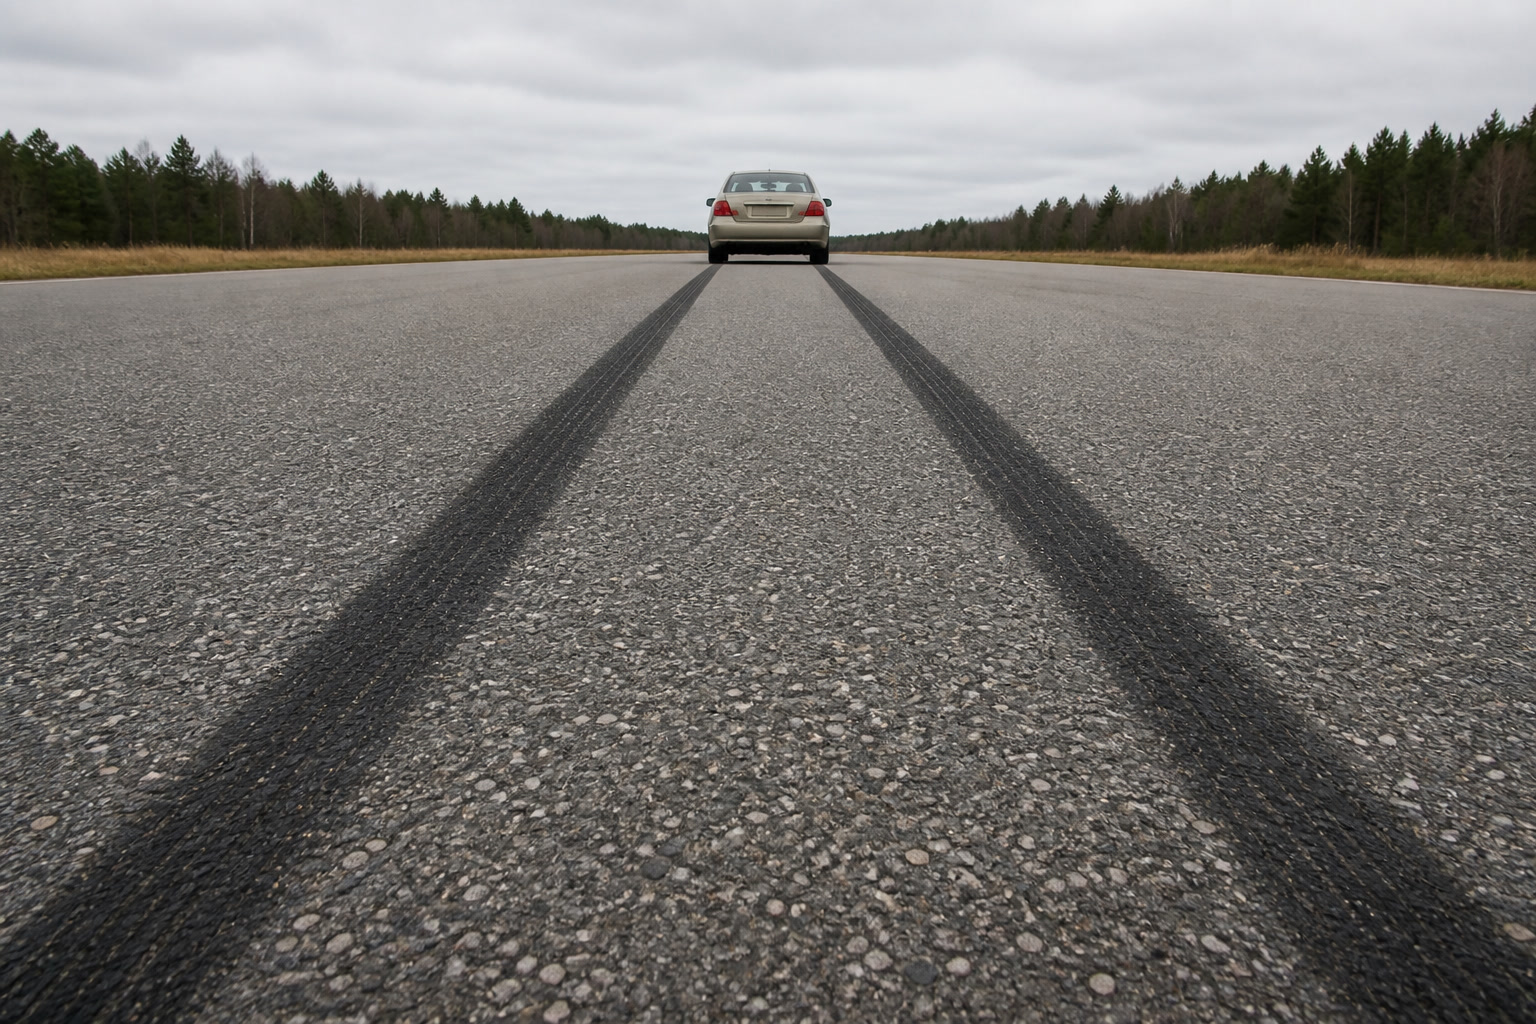
\includegraphics[width=0.55\linewidth]{images/book1/ai/g9-kinetic-skid-marks.jpg}

{\small Où est passée l'\omterm{prop:g9:kinetic-energy-safety:formula}{énergie cinétique}~: les freins et la route l'ont changée en \omterm{def:g5:heat-and-insulation:heat}{chaleur}, et les pneus ont signé le reçu.}
\end{omfigure}

\section{La distance d'arrêt}

\begin{proposition}[S'arrêter, c'est réfléchir puis freiner]\label{prop:g9:kinetic-energy-safety:stopping}
Un \omterm{def:g4:conductors-insulators:conductor}{conducteur} qui repère un danger ne s'arrête qu'après deux portions
de route~:
\begin{enumerate}
  \item la \emph{distance de réaction}\index{distance de réaction}~:
        la route parcourue pendant que le cerveau remarque et que le
        pied bouge --- environ une seconde entière à \omterm{def:g7:motion-average-speed:formula}{vitesse}
        inchangée, si bien que cette portion croît
        \emph{proportionnellement} à $v$~;
  \item la \emph{distance de freinage}\index{distance de freinage}~:
        la route dont les freins ont besoin pour mettre l'\omterm{prop:g9:kinetic-energy-safety:formula}{énergie
        cinétique} à la retraite --- et puisque $E_k$ porte $v^2$,
        cette portion croît avec le \emph{carré} de la \omterm{def:g7:motion-average-speed:formula}{vitesse}~:
        \omterm{def:g7:motion-average-speed:formula}{vitesse} doublée, route de freinage quadruplée.
\end{enumerate}
Leur somme, la \emph{distance d'arrêt}, est le nombre qui rencontre
l'enfant qui court après son ballon.
\end{proposition}

\begin{example}[Le tableau que tout conducteur devrait posséder]\label{ex:g9:kinetic-energy-safety:table}
Route sèche, \omterm{def:g4:conductors-insulators:conductor}{conducteur} attentif (une seconde de réaction~; bons
freins)~:
\begin{center}
\begin{tabular}{l|c|c|c}
\omterm{def:g7:motion-average-speed:formula}{vitesse} & réaction & freinage & arrêt \\
\hline
\qty{50}{km/h} & \qty{14}{m} & \qty{13}{m} & \qty{27}{m} \\
\qty{90}{km/h} & \qty{25}{m} & \qty{40}{m} & \qty{65}{m} \\
\qty{130}{km/h} & \qty{36}{m} & \qty{85}{m} & \qty{121}{m}
\end{tabular}
\end{center}
Lis-le deux fois. À \omterm{def:g7:motion-average-speed:formula}{vitesse} de ville, une longueur d'autobus et
demie~; à \omterm{def:g7:motion-average-speed:formula}{vitesse} d'autoroute, une piste d'athlétisme entière et un
cinquième. Et les proportions confirment les deux lois~: la réaction
croît comme $v$, le freinage comme $v^2$ --- à grande \omterm{def:g7:motion-average-speed:formula}{vitesse}, le
freinage dévore le total.
\end{example}

\begin{method}[Estimer une distance d'arrêt]\label{met:g9:kinetic-energy-safety:estimate}
\begin{enumerate}
  \item convertir la \omterm{def:g7:motion-average-speed:formula}{vitesse} en \unit{m/s} (diviser les
        \unit{km/h} par $3.6$)~;
  \item \omterm{prop:g9:kinetic-energy-safety:stopping}{distance de réaction}~: le trajet d'une seconde --- le
        nombre en \unit{m/s} lui-même, en \omterm{def:g2:measuring-length:units}{mètres}~;
  \item \omterm{prop:g9:kinetic-energy-safety:stopping}{distance de freinage}~: mettre un repère connu à l'échelle
        du carré --- à partir de \qty{13}{m} à \qty{50}{km/h},
        multiplier par $(v/50)^2$~;
  \item additionner, et comparer à ce que la route offre
        réellement devant soi.
\end{enumerate}
Une route mouillée double la part du freinage~; un \omterm{def:g4:conductors-insulators:conductor}{conducteur} fatigué
ou distrait étire la seconde de réaction vers deux --- refais la somme
avec les entrées honnêtes.
\end{method}

\begin{example}[Le prix d'un coup d'œil]\label{ex:g9:kinetic-energy-safety:glance}
Un coup d'œil de deux secondes sur un téléphone à \qty{90}{km/h}~: la
voiture parcourt $2 \times 25 = \qty{50}{m}$ --- un demi-terrain de
football --- conduits à l'aveugle, avant même que ne commence la
moindre seconde de réaction. À \omterm{def:g7:motion-average-speed:formula}{vitesse} de ville, le même coup d'œil
dépense en aveugle \qty{28}{m}~: au-delà du carrefour, au-delà du
portail de l'école. Le composant le plus dangereux de la voiture n'est
mesuré par aucune formule d'ici~: l'attention du \omterm{def:g4:conductors-insulators:conductor}{conducteur}.
\end{example}

\begin{remark}[Ceintures, coussins et casques]\label{rem:g9:kinetic-energy-safety:belts}
Dans une collision, la voiture s'arrête sur un \omterm{def:g2:measuring-length:units}{mètre} de tôle froissée
--- mais un passager non ceinturé continue à pleine \omterm{def:g7:motion-average-speed:formula}{vitesse} (la phrase
tranquille du chapitre précédent, sinistrement appliquée) jusqu'à être
arrêté par ce qui se présente~: tableau de bord, pare-brise, route.
Les ceintures et les coussins gonflables arrêtent le corps sur une
distance et une \omterm{def:g2:measuring-time:duration}{durée} plus longues et mettent son \omterm{prop:g9:kinetic-energy-safety:formula}{énergie cinétique} à
la retraite en douceur plutôt que d'un seul coup~; le casque du
cycliste en fait autant pour le contenu irremplaçable du crâne, sa
mousse écrasable achetant des \omterm{def:g2:measuring-length:units}{centimètres} d'arrêt en douceur. Aucun
d'eux ne réduit ton $E_k$ d'un seul \omterm{def:g9:kinetic-energy-safety:joule}{joule} --- ils civilisent sa
retraite.
\end{remark}

\section{Exercices}

\begin{exercise}[$\star$]\label{exo:g9:kinetic-energy-safety:1}
Donne l'\omterm{def:g6:measurement-in-science:measuring}{unité} d'\omterm{def:g5:everyday-energy:energy}{énergie} et deux de ses repères, et écris la formule de
l'\omterm{prop:g9:kinetic-energy-safety:formula}{énergie cinétique} avec ses \omterm{def:g6:measurement-in-science:measuring}{unités}.
\end{exercise}

\begin{exercise}[$\star$]\label{exo:g9:kinetic-energy-safety:2}
Calcule $E_k$~: un lièvre de \qty{2}{kg} à \qty{10}{m/s}~; un joueur
de rugby de \qty{80}{kg} à \qty{5}{m/s}.
\end{exercise}

\begin{exercise}[$\star$]\label{exo:g9:kinetic-energy-safety:3}
Qu'est-ce qui augmente le plus l'$E_k$ d'une voiture~: ajouter en
chargement la moitié de sa \omterm{def:g3:measuring-mass:mass}{masse}, ou augmenter sa \omterm{def:g7:motion-average-speed:formula}{vitesse} de moitié~?
Montre les deux facteurs.
\end{exercise}

\begin{exercise}[$\star$]\label{exo:g9:kinetic-energy-safety:4}
Nomme les deux portions de la distance d'arrêt et leurs lois de
croissance --- l'une proportionnelle, l'autre au carré.
\end{exercise}

\begin{exercise}[$\star$]\label{exo:g9:kinetic-energy-safety:5}
D'après le tableau du \omterm{def:g4:conductors-insulators:conductor}{conducteur}~: quelle fraction de la distance
d'arrêt est du freinage à \qty{50}{km/h} --- et à \qty{130}{km/h}~?
Qu'est-ce qui a changé~?
\end{exercise}

\begin{exercise}[$\star$]\label{exo:g9:kinetic-energy-safety:6}
Où passe l'\omterm{prop:g9:kinetic-energy-safety:formula}{énergie cinétique} d'une voiture qui freine~? Cite l'odeur
et le rougeoiement --- et la loi de l'enfance qui lui interdit de
simplement s'évanouir.
\end{exercise}

\begin{exercise}[$\star$]\label{exo:g9:kinetic-energy-safety:7}
Calcule la \omterm{prop:g9:kinetic-energy-safety:stopping}{distance de réaction} à \qty{36}{km/h}, \qty{72}{km/h} et
\qty{108}{km/h} (une seconde d'un \omterm{def:g4:conductors-insulators:conductor}{conducteur} attentif). À quel motif
simple les réponses obéissent-elles~?
\end{exercise}

\begin{exercise}[$\star$]\label{exo:g9:kinetic-energy-safety:8}
Pourquoi une ceinture de sécurité ne réduit-elle pas ton \omterm{prop:g9:kinetic-energy-safety:formula}{énergie
cinétique} --- et que civilise-t-elle à la place~?
\end{exercise}

\begin{exercise}[$\star\star$]\label{exo:g9:kinetic-energy-safety:9}
La \omterm{prop:g9:kinetic-energy-safety:stopping}{distance de freinage} d'un scooter vaut \qty{8}{m} à
\qty{30}{km/h}. Estime-la à \qty{60}{km/h} et à \qty{90}{km/h} --- et
énonce la loi qui t'a servi de facteur d'échelle.
\end{exercise}

\begin{exercise}[$\star\star$]\label{exo:g9:kinetic-energy-safety:10}
Des conseils municipaux abaissent la limitation aux abords des écoles
de \qty{50}{} à \qty{30}{km/h}. Compare les deux distances d'arrêt
(repère~: \qty{13}{m} de freinage à $50$~; une seconde de réaction)
--- et les deux \omterm{prop:g9:kinetic-energy-safety:formula}{énergies cinétiques}. Laquelle des deux comparaisons
te paraît la plus convaincante sur une affiche~?
\end{exercise}

\begin{exercise}[$\star\star$]\label{exo:g9:kinetic-energy-safety:11}
La pluie double les \omterm{prop:g9:kinetic-energy-safety:stopping}{distances de freinage}. Reconstruis la colonne
«~arrêt~» du tableau du \omterm{def:g4:conductors-insulators:conductor}{conducteur} pour route mouillée à $50$ et
\qty{90}{km/h} --- quelle composante as-tu doublée, laquelle non, et
pourquoi~?
\end{exercise}

\begin{exercise}[$\star\star\star$]\label{exo:g9:kinetic-energy-safety:12}
Un camion de \qty{20000}{kg} roule à \qty{90}{km/h}. Calcule son $E_k$
en notation scientifique~; trouve la \omterm{def:g7:motion-average-speed:formula}{vitesse} à laquelle une voiture de
\qty{1000}{kg} égalerait cette \omterm{def:g5:everyday-energy:energy}{énergie} (égale les deux formules ---
l'algèbre est tienne cette année)~; et conclus sur la raison d'être
des lits d'arrêt pour camions en perdition sur les routes de
montagne, alors qu'aucun lit de ce genre ne sert aux voitures.
\end{exercise}

\section{Problème~: la campagne de sécurité}

\begin{problem}[{Problème du week-end --- la classe conçoit la
campagne de sécurité routière de la commune~; des affiches vérifiées
par la formule~; les questions difficiles du
maire}]\label{pb:g9:kinetic-energy-safety:1}
La commune commande une campagne, à une condition~: tout nombre de
toute affiche doit survivre à un audit de physique. La classe calcule.
(Repères~: une seconde de réaction~; \qty{13}{m} de freinage à
\qty{50}{km/h}, à mettre à l'échelle du carré~; \omterm{def:g3:measuring-mass:mass}{masse} de la voiture
\qty{1000}{kg}.)

\medskip\noindent\textbf{Partie I --- affiche numéro un~: «~50, pas
60~».}
\begin{enumerate}
  \item Calcule les deux \omterm{def:g7:motion-average-speed:formula}{vitesses} en \unit{m/s} (une décimale).
  \item Les \omterm{prop:g9:kinetic-energy-safety:stopping}{distances de réaction} aux deux \omterm{def:g7:motion-average-speed:formula}{vitesses}~?
  \item Les \omterm{prop:g9:kinetic-energy-safety:stopping}{distances de freinage} aux deux (mets le repère à
        l'échelle)~?
  \item Le titre de l'affiche~: «~Dix \omterm{def:g6:measurement-in-science:measuring}{unités} de \omterm{def:g7:motion-average-speed:formula}{vitesse} en plus ---
        combien de \omterm{def:g2:measuring-length:units}{mètres} d'arrêt en plus~?~» Remplis le nombre.
\end{enumerate}

\medskip\noindent\textbf{Partie II --- affiche numéro deux~: «~le
mur de la \omterm{def:g7:motion-average-speed:formula}{vitesse}~».}
La maquette montre les \omterm{def:g5:everyday-energy:energy}{énergies} de choc sous forme de hauteurs de
chute~: un choc à la \omterm{def:g7:motion-average-speed:formula}{vitesse} $v$ «~équivaut~» à une chute depuis la
hauteur où la même \omterm{def:g5:everyday-energy:energy}{énergie} serait acquise.
\begin{enumerate}[resume]
  \item Calcule l'$E_k$ de la voiture à \qty{50}{km/h} (d'après la
        partie I) et à \qty{90}{km/h}.
  \item Les graphistes ont besoin de hauteurs~: une chute de
        \qty{1}{m} donne environ \qty{9.8}{kJ} à cette voiture
        ($m g h$ --- l'autre formule du chapitre suivant, empruntée
        en avance). À quelles hauteurs de chute correspondent les
        deux \omterm{def:g5:everyday-energy:energy}{énergies} de choc~? (Divise~; arrondis au \omterm{def:g2:measuring-length:units}{mètre}.)
  \item Quels bâtiments familiers correspondent à ces hauteurs~?
        Rédige la ligne de l'affiche.
  \item Le maire objecte~: «~Personne ne fonce dans un mur~; les
        voitures se froissent, les ceintures retiennent.~» Défends
        la physique de l'affiche tout en lui concédant son point
        --- que changent les zones de déformation et les
        ceintures, et quel nombre ne changent-elles pas~?
\end{enumerate}

\medskip\noindent\textbf{Partie III --- affiche numéro trois~: «~une
seconde~».}
\begin{enumerate}[resume]
  \item À \qty{90}{km/h}, combien de \omterm{def:g2:measuring-length:units}{mètres} coûte une seconde de
        distraction avant tout freinage~? Et un coup d'œil de deux
        secondes sur le téléphone~?
  \item La variante du \omterm{def:g4:conductors-insulators:conductor}{conducteur} fatigué~: réaction étirée à deux
        secondes. Recalcule la distance d'arrêt complète à
        \qty{90}{km/h} et compare aux \qty{65}{m} du \omterm{def:g4:conductors-insulators:conductor}{conducteur}
        attentif.
  \item Un conseiller sceptique~: «~Une seconde pèse sûrement peu
        à côté de ces gros nombres de freinage.~» À quelles
        \omterm{def:g7:motion-average-speed:formula}{vitesses} a-t-il le plus tort --- basses ou hautes~?
        (Compare les lois de croissance des deux composantes.)
  \item Signe la campagne~: trois lignes de bas d'affiche, une par
        affiche, portant chacune sa formule en mots simples.
\end{enumerate}
\end{problem}
